\documentclass{standalone}
\usepackage{../../../../preamble_general}
\usepackage{../../../../preamble_tikz}
\usepackage{../../../../preamble_math}


\begin{document}
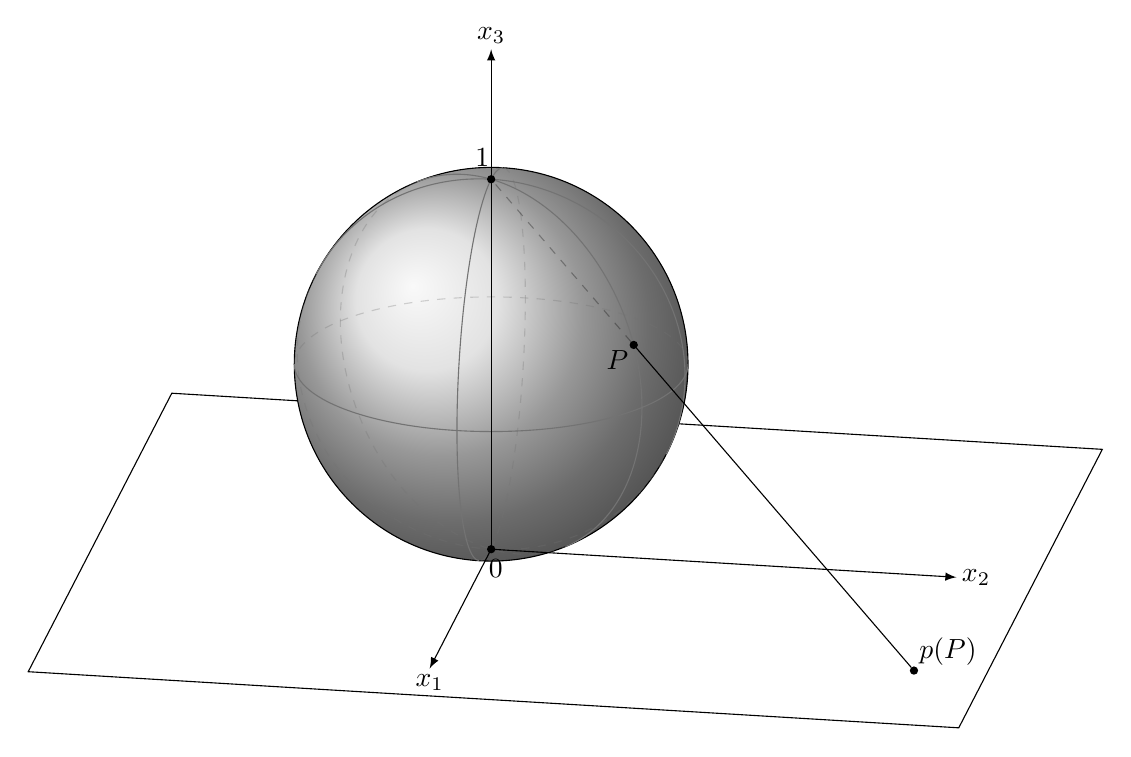
\begin{tikzpicture}
  \newcommand\pgfmathsinandcos[3]{%
    \pgfmathsetmacro#1{sin(#3)}%
    \pgfmathsetmacro#2{cos(#3)}%
  }
  \newcommand\LongitudePlane[3][current plane]{%
    \pgfmathsinandcos\sinEl\cosEl{#2} % elevation
    \pgfmathsinandcos\sint\cost{#3} % azimuth
    \tikzset{#1/.estyle={cm={\cost,\sint*\sinEl,0,\cosEl,(0,0)}}}
  }
  \newcommand\LatitudePlane[3][current plane]{%
    \pgfmathsinandcos\sinEl\cosEl{#2} % elevation
    \pgfmathsinandcos\sint\cost{#3} % latitude
    \pgfmathsetmacro\yshift{\cosEl*\sint}
    \tikzset{#1/.estyle={cm={\cost,0,0,\cost*\sinEl,(0,\yshift)}}} %
  }
  \newcommand\DrawLongitudeCircle[2][1]{
    \LongitudePlane{\angEl}{#2}
    \tikzset{current plane/.prefix style={scale=#1}}
    % angle of "visibility"
    \pgfmathsetmacro\angVis{atan(sin(#2)*cos(\angEl)/sin(\angEl))} %
    \draw[current plane,gray!90!black] (\angVis:1) arc (\angVis:\angVis+180:1);
    \draw[current plane,dashed,gray!90!black,opacity=0.3] (\angVis-180:1) arc (\angVis-180:\angVis:1);
  }
  \newcommand\DrawLatitudeCircle[2][1]{
    \LatitudePlane{\angEl}{#2}
    \tikzset{current plane/.prefix style={scale=#1}}
    \pgfmathsetmacro\sinVis{sin(#2)/cos(#2)*sin(\angEl)/cos(\angEl)}
    % angle of "visibility"
    \pgfmathsetmacro\angVis{asin(min(1,max(\sinVis,-1)))}
    \draw[current plane,gray!90!black] (\angVis:1) arc (\angVis:-\angVis-180:1);
    \draw[current plane,dashed,gray!90!black,opacity=0.3] (180-\angVis:1) arc (180-\angVis:\angVis:1);
  }

  \tikzset{%
    >=latex, % option for nice arrows
    inner sep=0pt,%
    outer sep=2pt,%
    mark coordinate/.style={inner sep=0pt,outer sep=0pt,minimum size=3pt,
        fill=black,circle}%
  }
  %% some definitions

  \def\R{2.5} % sphere radius
  \def\angEl{20} % elevation angle
  \def\angAz{-100} % azimuth angle
  \def\angPhi{-40} % longitude of point P
  \def\angBeta{19} % latitude of point P

  %% working planes

  \pgfmathsetmacro\H{\R*cos(\angEl)} % distance to north pole
  \tikzset{xyplane/.estyle={cm={cos(\angAz),sin(\angAz)*sin(\angEl),-sin(\angAz),
            cos(\angAz)*sin(\angEl),(0,-\H)}}}
  \LongitudePlane[xzplane]{\angEl}{\angAz}
  \LongitudePlane[pzplane]{\angEl}{\angPhi}
  \LatitudePlane[equator]{\angEl}{0}

  %% draw xy-plane and sphere

  \draw[xyplane] (-2*\R,-2*\R) rectangle (2.2*\R,2.8*\R);
  \fill[ball color=gray!30] (0,0) circle (\R); % 3D lighting effect
  \draw (0,0) circle (\R);

  %% draw meridians and latitude circles

  \DrawLatitudeCircle[\R]{0} % equator
  \DrawLongitudeCircle[\R]{\angAz} % xz-plane
  \DrawLongitudeCircle[\R]{\angAz+90} % yz-plane
  \DrawLongitudeCircle[\R]{\angPhi} % pz-plane

  %% characteristic points

  \coordinate (O) at (0,0);
  \coordinate[mark coordinate] (N) at (0,\H);
  \coordinate[mark coordinate] (S) at (0,-\H);
  \path[pzplane] (\angBeta:\R) coordinate[mark coordinate] (P);
  \path[pzplane] (\R,0) coordinate (PE);
  \path[xzplane] (\R,0) coordinate (XE);
  \path (PE) ++(0,-\H) coordinate (Paux); % to aid Phat calculation
  \coordinate[mark coordinate] (Phat) at (intersection cs: first line={(N)--(P)},
  second line={(S)--(Paux)});

  %% draw xyz coordinate system

  \draw[xyplane,<->] (1.8*\R,0) node[below] {$x_1$} -- (0,0) -- (0,2.4*\R)
  node[right] {$x_2$};
  \draw[->] (0,-\H) -- (0,1.6*\R) node[above] {$x_3$};

  %% draw lines and put labels

  \draw[\ana,dashed,opacity=0.3] (P) -- (N) +(0.3ex,0.6ex) node[above left,black,opacity=1] {$1$};
  \draw[\ana] (P) -- (Phat) node[above right,black] {$p(P)$};
  \path (S) +(0.4ex,-0.4ex) node[below] {$0$};
  \draw (P) node[below left] {$P$};
  \draw (-3,-2,2) node[below left,scale=2] {$\CC$};
\end{tikzpicture}
\end{document}